\documentclass{article}

\usepackage[francais]{babel}
\usepackage{hyperref}
\usepackage[latin1]{inputenc}
\usepackage{graphicx}
\usepackage{listings}

\title{Rapport de stage - Coloane}
\date{Janvier 2008}
\author{Monir CHAOUKI}

\begin{document}

\maketitle

\begin{quotation}
\textit{
Le but de mon stage est, la conc�ption d'un point d'extension, et la r�alisation 
d'une extension pour Coloane. La conc�ption de points d'extensions, permettra � 
Coloane, d'int�grer de nouvelles fonctionalit�s, via les contributions 
d'autres d�veloppeurs (en respectant certaines conditions), sans que ceux--ci,
 est � modifier le code de Coloane.}

\end{quotation}

\newpage
\section{Notions impotrtantes}
Nous allons pr�senter quelques notions, avant de passer � la pr�sentation de 
Coloane, et aux m�canismes mis en jeu pour la conception et � la r�alisation 
d'un point d'extension.

\subsection{Plugin}
Un plugin, est un programme qui s'ajoute � une application principale, pour lui 
offrire de nouvelles fonctionnalit�s. Il existe plusieurs applications qui 
proposent d'ajouter des plugins. Par exemples, le navigateur internet 
"Mozilla FireFox", propose plusieurs plugins allant du simple traducteur, aux 
lecteur de MP3 int�gr� au navigateur. Tous ces plugins sont issus des 
contributions de developpeurs.

\subsection{Extensions}
Une extension peut �tre vue comme un plugin limit�. En faite, une extension, 
permet d'ajouter de nouveaux services, � une fonctionnalit� d�j� pr�sente dans 
une application. Reprenons notre pr�c�dent exemple sur le navigateur internet 
"Mozilla FireFox". Comme il a �t� dit plus haut, "Mozilla FireFox" proposent 
des plugins qui permettent de traduire des pages, dans une langue sp�cifique. 
Il est possible, si les plugins le permettent, d'ajouter de nouvelle langue au 
traducteur, via les contributions d'autres developpeurs, si ceux--ci developpent 
un extensions qui s'ajoute aux plugins existant.

\subsection{Points d'extensions}
Nous avons vue, qu'une extension, est un service qui venai s'ajouter aux 
fonctionnalit�s, d'une application (ou d'un plugin). Pour qu'une extension 
puisse s'ajoute � une application (ou � un plugin), il faut que celle--ci 
d�clare un point d'extension. La d�claration de points d'extensions, permet 
ainssi, � une application d'�tre extensible, et d'offrire de nouveaux services, 
venant d'autres contributions. Donc, un point d'extension, permet d'indiquer, 
aux extensions o� elle doivent venire se greffer, pour qu'elle puisse enrichire 
une application (ou un plugin).

\newpage
\section{Coloane}

\subsection{Presentation de Coloane}
Coloane est un plugin, pour Eclipse, qui permet de mod�liser, les r�seaux de 
Petri. L'une de ses philosophies est d'�tre multi--platforme. Le moteur 
physique, utilise un format non standard, le CAMI, pour travailler, sur ces 
r�seaux de Petri. 

\subsection{Evolutions de Coloane}
L'une des �volutions tr�s impotrantes, � mettre en place pour Coloane, c'est 
d'offrire la possiblit� d'utilsier diff�rents formats de repr�sentations de 
r�seau de Petri, permettant ainssi l'�change de diff�rents formats de fichiers.

En effet, aujourd'hui, l'inconveniant majeur de Coloane commme nous l'avons 
�crit plus haut, c'est qu'il n'utilisent qu'un format, non standardiser le: 
CAMI. Or, il existe plusieurs formats pour la repr�sentation des r�seaux de 
Petri, dont un principale en cours de normalisation le: PNML.

\subsection{Limites li�s aux l'evolutions de Coloane}
Aujourd'hui, il est biens�re possible de faire �voluer Coloane, mais cela 
implique d'entrer � l'int�rieur du code, et de le modifier directement pour 
ajouter les �volutions voulus.

Or, le fait d'entrer dans le code, de Coloane, qui est actuelement stable, est 
un facteur important d'apparition de bugs. De plus, si plusieurs d�veloppeurs 
souhaitent contribuer au projet Coloane pour le faire �voluer, le code risque 
vite d'�tre confus, sans r�gles etablies.

Il serait donc, int�resant de pouvoire faire �voluer Coloane, sans toucher 
au code. Le fait de faire �voluer Coloane correspondrait, � ajouter de 
nouvelles fonctionnalit�es ou de nouveaux services. Or, ajouter des 
fonctionnalit�es ou services, c'est ajouter un plugin ou une extension.

Par cons�quant, si l'on veut faire evoluer Coloane, il faudrait 
songer � utiliser des plugins qui se mettent � coter de lui, ou des extensions 
qui viennent se greffer � lui.

\newpage
\section{Conv�rtiseur de formats de repr�sentations de R�seau de Petri}
Nous avons vue pr�cedement, que l'une des �volutions importantes pour 
Coloane, � mettre en place, est un conv�rtiseur de format de repr�sentations de 
R�seau de Petri, permettant ainssi � Coloane d'importer et exporter diff�rents 
formats dont, le plus importants le: PNML.

\subsection{Solutitions envisag�es}
Comme nous l'avons �cris, deux solutions sont envisagales pour permettre � 
Coloane d'integr� de nouvelle fonctionnalit�s et d'�tre �volutif (i.e. int�grer 
de nouveaux formats): un plugin ou un point d'extension.

\subsubsection{le plugin}
Dans le cas d'un plugin, Coloane, n'aura aucune mettrise au niveau de 
l'int�rface graphique qui permet d'int�ragir avec l'utlisateur pour 
l'importations et l'exportations de nouveaux format . Toutes les contributions 
pourrons g�rer l'int�rface graphique,et implementer les fonctions d'importations 
et d'exportations de nouveaux format, comme bon leurs semblent.

\subsubsection{le point d'extension}
Dans le cas d'un point d'extension, Coloane g�rera toujours l'int�rface 
graphique, mais d�l�guera aux extensions qui viendront se greffer sur ce point, 
seulement, les fonctions d'importations et d'exportations de nouveaux formats et 
ceux--ci devrons respecter certaines r�gles.

\subsection{Solutions choisies}
Il est bien �vident que nous allons choisir d'utiliser un point d'extension dans 
Coloane pour que l'on est un certaines ma�trise, des contributions qui permetteront 
de faire des importations et des exportations de nouveaux format.

En effet, chaque contributions devrons avoir la m�me int�race graphique pour 
interagire avec l'utilisateur, pour que celui--ci, ne soit pas perturber 
lorsqu'il veut exporter ou importer dans des formats difff�rent. De plus, on 
imposera aux contributions de respecter certaines r�gles qui est en faites: 
une int�rfaces � implementer.

Ainssi toutes nouvelles contributions offrants de nouveaux format n'aura qu' � 
offrire ses service en utilisant le point d'extension d�finie par Coloane.


\newpage
\section{Pr�cisions sur les points d'extensions de Coloane}
Nous allons utiliser des points d'extensions, comme nous l'avons expliqu�s pr�cedement, 
pour permettre aux contributions d'offrire leur services d'importations et 
d'exportations. Utiliser des points d'extensions impliquent de pr�parer Coloane. Pour cela, 
il faut ajouter quelques lignes dans le fichier \textbf{plugin.xml} pour d�finire les points 
d'extensions, cr�er les fichiers \textbf{imports.exsd} et \textbf{imports.exsd } dans un 
repertoire \textbf{schema/} qui d�finissent la grammaire des points d'extensions, et 
modifier le fichier \textbf{MANIFEST.MF} pour lui sp�cifier les packages � exporter et 
qui sont suc�ptibles d'�tre utilis�s par les extensions.

Une remarque importante, Eclipse offre une int�rface graphique tr�s agr�able : 
PDE (Plug-ins Development Environment), qui permet  la conc�ption et la definition de points d'extensions sont 
diffucl�es.

\subsection{\textbf{plugin.xml}}
Dans le fichier \textbf{plugin.xml}, il faut juste d�finire les points d'extensions 
qui existent pour le plugin Coloane, ici nous avons avons d�cal� deux points
d'extensions: \textit{Imports} et \textit{Exports}. En effet les contributions ne sont oblig�es d'implementer � la fois 
les fonctions d'importatios et d'exportations.

Voicie, les deux lignes ajout�es dans le fichier \textbf{plugin.xml}:
\begin{verbatim}
<extension-point id="exports" name="Exports" schema="schema/exports.exsd"/>
<extension-point id="imports" name="Imports" schema="schema/imports.exsd"/>
\end{verbatim}

\subsection{\textbf{imports.exsd} et \textbf{exports.exsd}}
Dans les fichiers \textbf{imports.exsd} et \textbf{exports.exsd}, on d�finie la grammaire des 
points d'extensions. Plus pr�cisement, le nom des attributs, et leur types. Cela permet 
d'indiquer comment utiliser ces points d'extensions. Dans notre cas nous avons trois attributs/
\begin{itemize}
  \item id: C'est l'identifiant du points d'extensions.
  \item name: C'est le nom du nom du point d'extension
  \item class: C'est l'int�rface que devrons implements les extensions
\end{itemize}
Noter, qu'il est tr�s facile, gr�ce au PDE (Plug-ins Development Environment), de cr�er ces fichiers, 
\textbf{imports.exsd} et \textbf{exports.exsd}. En effet, il n'y a qu'� remplire des champs, et le PDE, se 
charge de g�n�rer automatiquement, les fichiers attendus.

\subsection{MANIFEST.MF}
Dans le fichier \textbf{MANIFEST.MF}, on doit d�finire les packages, que l'on doit exporter 
pour que les extensions puissent y avoir acc�s, afin d'impl�menter les fonctions 
d'importation et d'exportation.

Voicie, un extrait du fichier \textbf{MANIFEST.MF}, pr�sentant, dans notre 
cas les packages export�s, qui definissent les exceptions que dervons lever les extensions, ainssi que les interfaces 
� implementer, et les methodes � utiliser pour cr�er un IModelImpl, etc...

\begin{verbatim}
Export-Package: fr.lip6.move.coloane.core.exceptions,
 fr.lip6.move.coloane.core.interfaces,
 fr.lip6.move.coloane.core.main,
 fr.lip6.move.coloane.core.motor.formalism,
 fr.lip6.move.coloane.core.ui.model
\end{verbatim}

\newpage
\section{Modifications apport�es � Coloane}
Nous avons vus approximativement, les modifications apport�es � Coloane, pour
d�clarer des points d'extensions. A pr�sent, nous allons pr�sent�s, les modifications 
au niveaux de l'int�rface utilisateur, et les classes ajout�es.

\subsection{L'int�rface utilisateur}
\subsubsection{Les items  \textit{"Imports From XXX..."} et \textit{"Exports To XXX..."}}
Comme, il sera dor�navant, possible d'ajouter diff�rents formats pour 
la repr�sentations de R�seau de Petri, il est inimaginable, qu'a chaque format XXX d'ajouter un 
des items \textit{Imports From XXX...} et \textit{Exports To XXX...}, dans le menu \textit{File}, 
cela devindrait trop gros.

Nous avons, donc, opt�s, pour seulement deux items \textit{Imports From...} et \textit{Exports To...}, 
dans le menu \textit{File}, qui permettent, d'ouvrire une boite de dialogue, et 
demandant � l'utilisateur de choisir un format, et le nom du fichier � importer, ou � exporter.

Pour cela, nous avons d�clarer, dans \textbf{plugin.xml}, deux itmes, pour \textit{Imports From...} et 
\textit{Exports To...}.

\begin{verbatim}
<actionSet
            id="fr.lip6.move.coloane.actionSet.file"
            label="%FILEACTIONS_ID"
            visible="true">
         <action
               class="fr.lip6.move.coloane.core.ui.actions.ExportTo"
               icon="resources/icons/export_wiz.gif"
               id="exportTo"
               label="%EXPORT_TO_ITEM"
               menubarPath="file/import.ext"
               style="push">
         </action>
         <action
               class="fr.lip6.move.coloane.core.ui.actions.ImportFrom"
               icon="resources/icons/import_wiz.gif"
               id="importFrom"
               label="%IMPORT_FROM_ITEM"
               menubarPath="file/import.ext"
               style="push">
         </action>
      </actionSet>
\end{verbatim}
On peut voire, que nous avons d�finie deux classe:
\begin{verbatim}
fr.lip6.move.coloane.core.ui.actions.ExportTo
fr.lip6.move.coloane.core.ui.actions.ImportFrom
\end{verbatim}
ces classes s�rvent � definre les actions � effectuer, lorsqu'un utilisateur appuie sur 
l'un de ces items. Il faut noter que ces classes peuvent �tre consid�rer comme g�nerique car 
elles sont capables de cr�er n'importe quelles instances pour importer ou exporter un format, en utilisant, 
\textbf{ExportToExtension} ou \textbf{ImportFromExtension}, nous y reviendrons, plus tard.

\subsubsection{Les bo�tes de dialogues}
La d�finitions des bo�tes de dialogues \textbf{ImportFrom} et \textbf{ExportTo}, sont faites dans
le package: 
\begin{verbatim}
fr.lip6.move.coloane.core.ui.dialogs
\end{verbatim}
Ces deux classes h�rites de:
\begin{verbatim}
org.eclipse.jface.dialogs.Dialog;
\end{verbatim}
On peut remarquer, que ces classes font appel � \textbf{ExportToExtension} ou \textbf{ImportFromExtension}, 
pour afficher la liste des formats disponibles, nous y reviendrons plus tard.

\subsection{Les contraintes pour les extensions}
Pour que Coloane, puissent exporter et importer de nouveaux format, il faut que les extensions qui impl�mentes, 
ces services, r�spectent certaines r�gles. Ces r�gles sont en faites des int�rfaces � impl�menter. Ici, nous avons 
deux interfaces:
\begin{verbatim}
fr.lip6.move.coloane.core.interfaces.IExportTo
fr.lip6.move.coloane.core.interfaces.IImportFrom
\end{verbatim}
ces int�rfaces permettent � Coloane, de faire appel aux methodes (qui doivent �tre commune � toutes les extensions), 
d'importations et d'exportations, quand l'utilisateur le demande, via les itmes correspondant.
\begin{verbatim}
public interface IExportTo {
	public void export(IModelImpl modeleCourant,String filePath) throws ColoaneException;
}

public interface IImportFrom {
	public IModelImpl importFrom(String filePath) throws ColoaneException;
}
\end{verbatim}
ces methodes sont utiliser par les classes:
\begin{verbatim}
fr.lip6.move.coloane.core.ui.actions.ExportTo
fr.lip6.move.coloane.core.ui.actions.ImportFrom
\end{verbatim}

\subsection{Comment savoire quelles extensions sont pr�sentes}
L'une des difficult�s, c'est de savoir quelles sont les extensions pr�sentent, 
pour pouvoir afficher leur nom dans la liste d�roulante des bo�te de dialogues et ainssi pouvoire cr�� une 
instance pour exporter ou importer le formats voulu par l'utilisateur.

Pour cela nous avons, cr�� les classes suivnates:
\begin{verbatim}
fr.lip6.move.coloane.core.extensions.ExportToExtension
fr.lip6.move.coloane.core.extensions.ImportFromExtension
\end{verbatim}
Ces classes possedent deux methodes:
\begin{itemize}
  \item \verb?getAllNameExtensionConvert?: cette m�thode est utiliser par les bo�tes de dialogues \textbf{ImportFromDialog} et \textbf{ExportToDialog}, pour 
afficher la listes des noms des extensions.
  \item \verb?createConvertInstance     ?: cette m�thode est utiliser 
par les classes qui \textbf{ImportFrom} et \textbf{ExportTo}, pour cr�� 
une instance pour exporter ou importer un format.
\end{itemize}


\newpage
\section{Conc�ption de points d'extensions}
Nous allons, vous pr�senter, comment cr�er un point d'extension, pour permttre � Coloane, d'int�grer via des contributions de nouveaux services d'exportations. Pour cela, nous allons utiliser le PDE (Plug--ins Developement Environment) pr�sent dans Eclipse.
 
\subsection{D�claration du point d'extension}
L'onglet 'Extension points' de l'�diteur de fichiers manifestes aide � la cr�ation 
de nouveaux points d'extension. Ouvrir cet onglet pour le plugin 'fr.lip6.move.coloane.core'. 
Le bouton 'Add...' ouvre un assistant permettant d'indiquer l'ID du nouveau point d'extension (l'ID r�el sera 
la concat�nation de l'ID du plugin et de la valeur de ce champ), son nom et le nom du fichier qui contiendra la grammaire :
\\
%%%%%%%%%%%
\includegraphics[width=1.00\textwidth]{images/pe1.jpg}
%%%%%%%%%%%

\subsection{D�finition de la grammaire}
Notre point d'extension doit permettre � des plugins de contribuer de nouveaux types de formats d'exportations. Nous proposons donc que la grammaire soit compos�e d'un �l�ment XML nomm� 'Exports' comprenant trois attributs 'id', 'nom' et 'classe'.

Cette grammaire doit �tre d�finie dans un fichier XMLSchema avec une extension .exsd. Le fichier a �t� cr�� automatiquement lors de l'�tape pr�c�dente et l'�diteur de fichiers .exsd a �t� ouvert sur notre fichier. L'�diteur dispose de plusieurs onglets, se placer dans l'onglet 'Definition' et utiliser le bouton 'Add Element' pour cr�er un �l�ment XML que nous nommerons 'Exports' :
\\
%%%%%%%%%%%
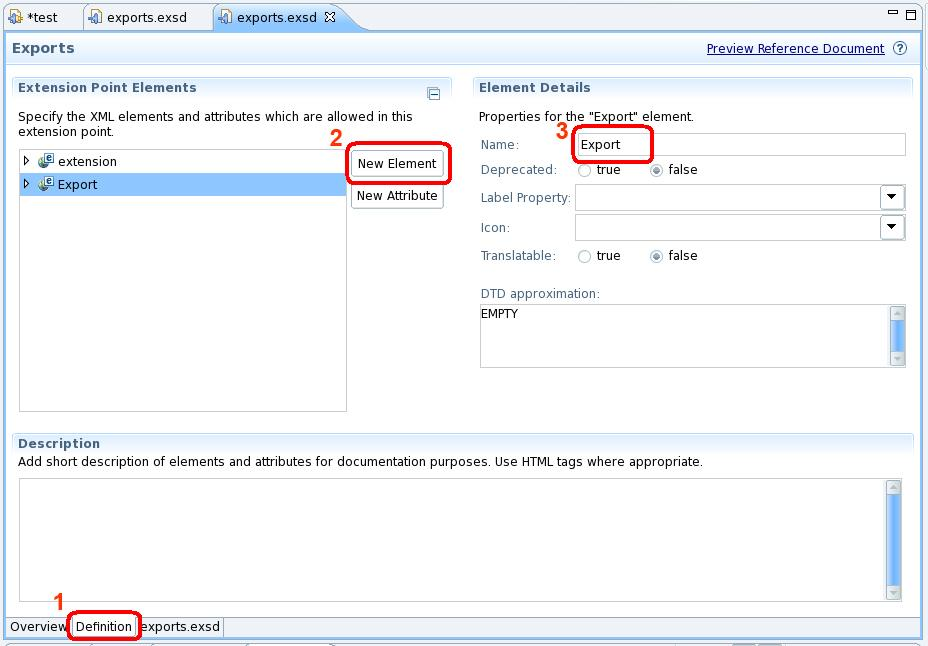
\includegraphics[width=1.00\textwidth]{images/pe2.jpg}
%%%%%%%%%%%
\\
\\
\\

Utiliser le bouton 'New Attribute' pour cr�er les attributs 'id' et 'nom'. Indiquer que ces attributs sont 'required' et de type 'string' :
\\
%%%%%%%%%%%
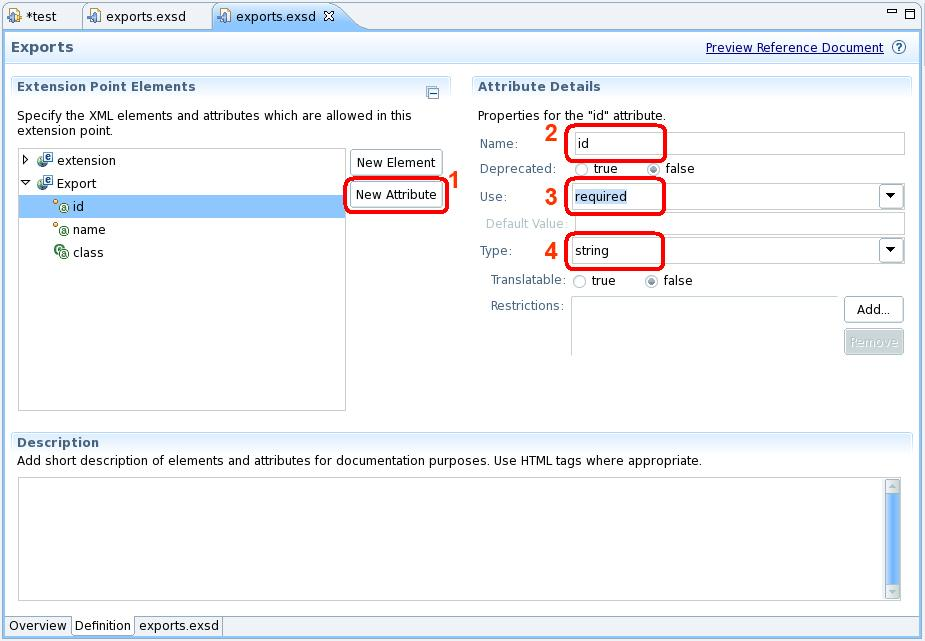
\includegraphics[width=1.00\textwidth]{images/pe3.jpg}
%%%%%%%%%%%
\\
\\
\\

Cr�er ensuite l'attribut 'classe'. Sp�cifier qu'il est 'required' et de type 'java'. Cet attribut sera utilis� par les plugins contributeurs pour indiquer le nom de la classe qui g�re l'exportation d'un format. Pour que notre plugin (celui d�finissant le point d'extension) puisse manipuler les classes fournies par les plugins contributeurs, nous allons leur imposer une interface commune. Le nom de cette interface est � indiquer dans le champ 'Implements' :
\\
%%%%%%%%%%%
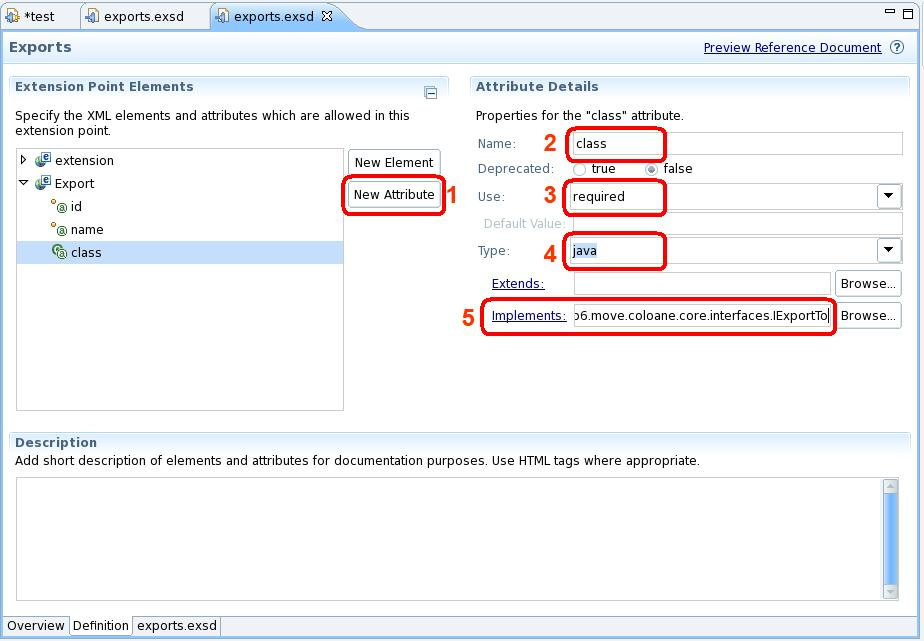
\includegraphics[width=1.00\textwidth]{images/pe4.jpg}
%%%%%%%%%%%
\\
\\
\\

Ajouter l'interface dans le plugin 'fr.lip6.move.coloane.core.interfaces', son code est le suivant


%\begin{verbatim}
\begin{lstlisting}[language=java]
package fr.lip6.move.coloane.core.interfaces;

import fr.lip6.move.coloane.core.exceptions.ColoaneException;
import fr.lip6.move.coloane.core.ui.model.IModelImpl;

public interface IExportTo {
	public void export(IModelImpl modeleCourant,String filePath) 
		throws ColoaneException;
}
\end{lstlisting}
%\end{verbatim}




Cette interface devra �tre utilisable par les plugins d�pendants : dans l'�diteur de fichier manifestes, s�lectionner l'onglet 'Runtime' et ajouter 
le package \\ 'fr.lip6.move.coloane.core.interfaces' dans la section 'Exported Packages'.



La grammaire d'un point d'extension se compose syst�matiquement d'un �l�ment parent nomm� 'extension'. Il nous faut indiquer la relation entre l'�l�ment 'extension' et notre �l�ment 'Export'. Dans notre cas l'�l�ment 'extension' peut contenir plusieurs sous-�l�ments 'Export' (un plugin peut fournir plusieurs types de formats d'exportations), pour d�finir ce lien il faut utiliser le menu contextuel sur l'�l�ment extension et s�lectionner 'New - Compositor - Sequence' :
\\
%%%%%%%%%%%
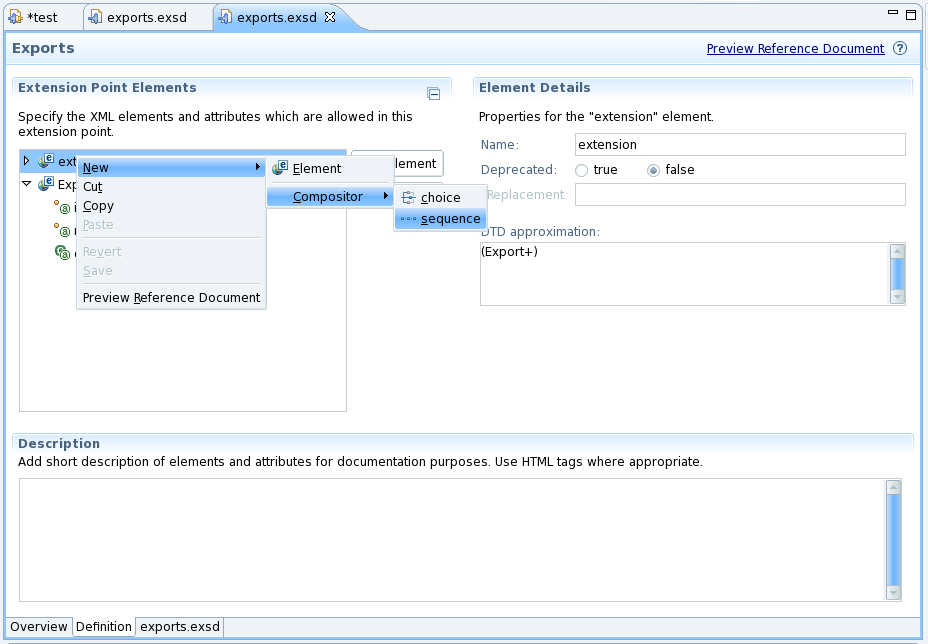
\includegraphics[width=1.00\textwidth]{images/pe5.jpg}
%%%%%%%%%%%
\\
\\
\\

Ouvrir ensuite le menu contextuel sur la s�quence et s�lectionner 'New - Reference - Export' :
\\
%%%%%%%%%%%
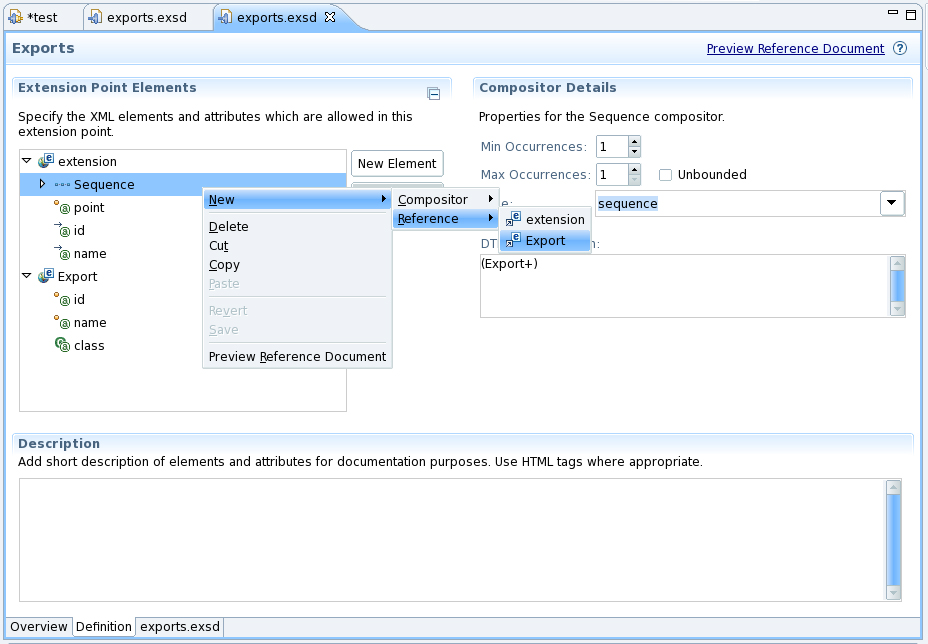
\includegraphics[width=1.00\textwidth]{images/pe6.jpg}
%%%%%%%%%%%
\\
\\
\\

S�lectionner la r�f�rence vers l'�lement 'Export' et cocher la case 'Unbounded' dans la partie de gauche:
\\
%%%%%%%%%%%
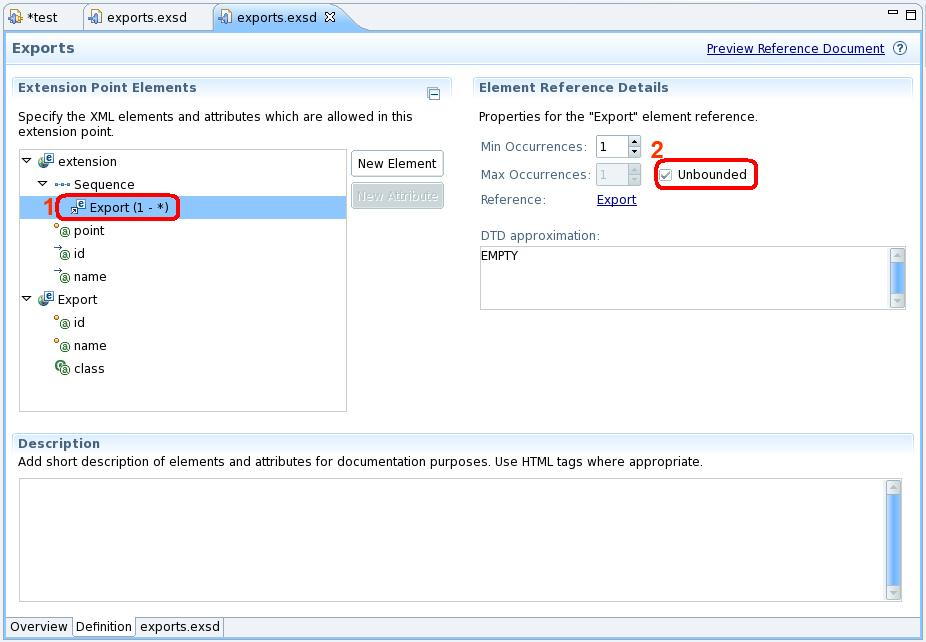
\includegraphics[width=1.00\textwidth]{images/pe7.jpg}
%%%%%%%%%%%
\\
\\
\\






















\newpage
\section{R�alisation d'une extension}
Pour r�aliser des extensions pour Coloane offrant de nouveaux services d'imporations ou d'exportations, 
il suffit d'utilis�, les points d'extensions que nous avons d�finie, pr�cedement.Ici, aussi gr�ce au, PDE, 
nous pouvons cr�er facilement des extensions.
Nous allons vous pr�senter la d�finition d'un extension permettant d'exporter au format DOT, en utilsant le PDE. 

\subsection{D�finition de l'extension \textbf{exportToDOT}}
Dans l'�diteur de fichiers manifestes de ce plugin, s�lectionner l'onglet 'Extensions'. 
Dans cet onglet cliquer sur le bouton 'Add...' : la liste de tous les points d'extension est pr�sent�e.
Dans l'assistant d�cocher la case 'Show only extension points from required plugins' et s�lectionner 
le point d'extension \textbf{fr.lip6.move.coloane.core.exports}:
%% AJOUTER IMAGE %%
\\
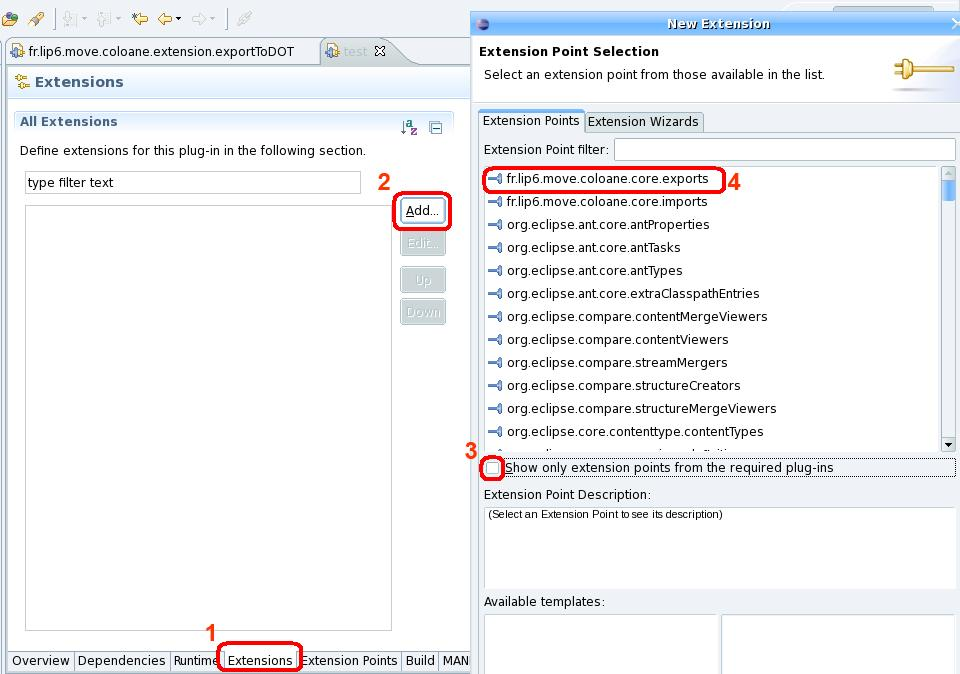
\includegraphics[width=1.00\textwidth]{images/ext1.jpg}
%% AJOUTER IMAGE %%
\\
\\
\\


L'objectif de l'onglet 'Extensions' est de g�n�rer la d�finition XML de 
l'extension dans le fichier plugin.xml. S�lectionner le point d'extension 
et utiliser le menu contextuel pour ajouter un des �l�ments XML d�clar�s dans 
la grammaire associ�e au point d'extension, dans notre cas un �l�ment de type 'Exports':
%% AJOUTER IMAGE %%
\\
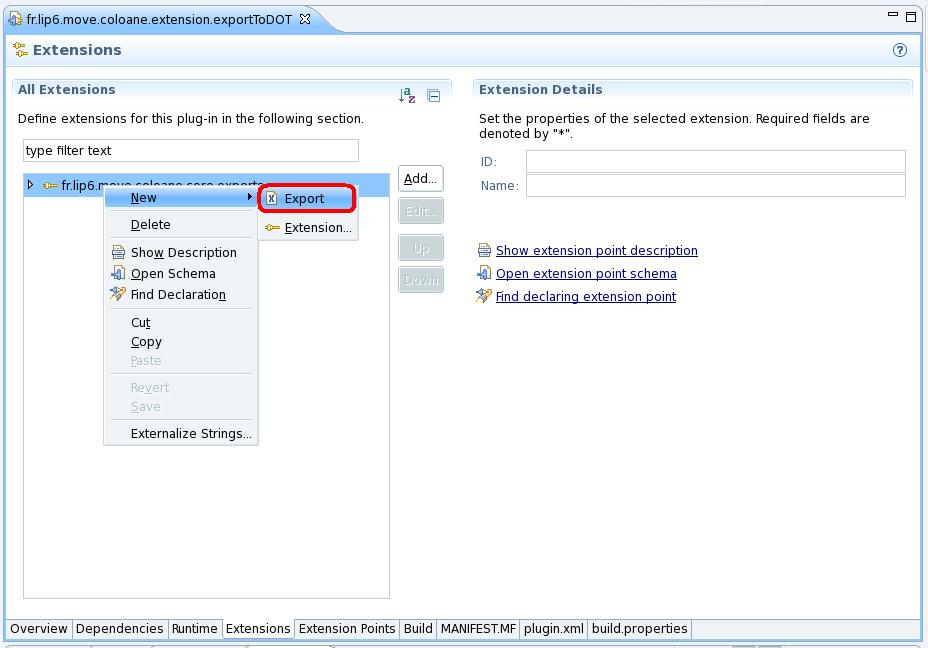
\includegraphics[width=1.00\textwidth]{images/ext2.jpg}
%% AJOUTER IMAGE %%
\\
\\
\\


La partie de gauche de l'�diteur permet de voir les attributs associ�s � cet 
�l�ment XML et d'indiquer leurs valeurs :
%% AJOUTER IMAGE %%
\\
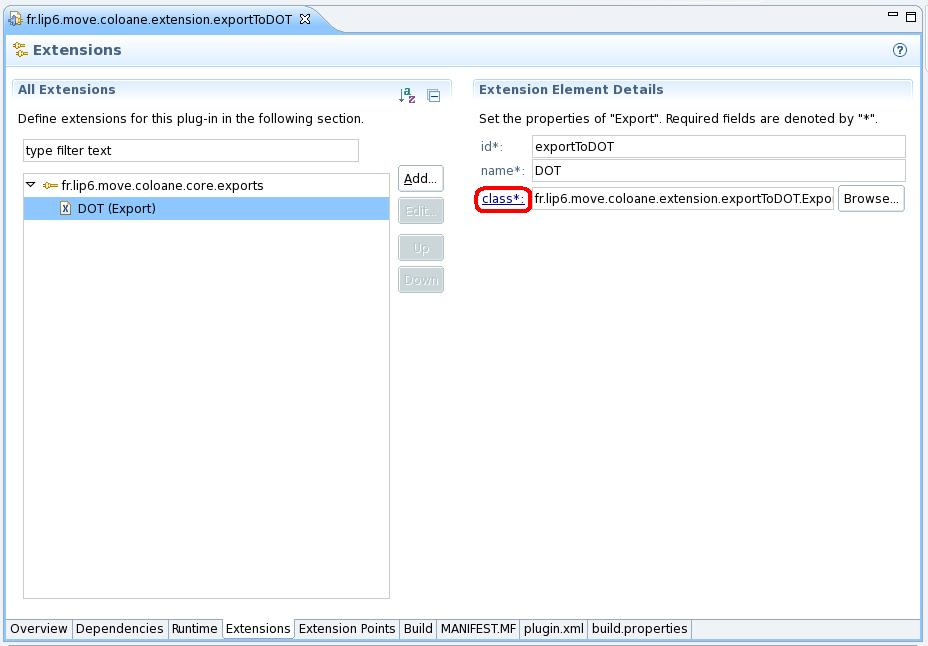
\includegraphics[width=1.00\textwidth]{images/ext3.jpg}
%% AJOUTER IMAGE %%
\\
\\
\\


La d�finition de notre extension est termin�e, le code XML correspondant a �t� g�n�r� dans le fichier plugin.xml :
\begin{verbatim}
<extension
         point="fr.lip6.move.coloane.core.exports">
      <Export
            class="fr.lip6.move.coloane.extension.exportToDOT.ExportToImpl"
            id="exportToDOT"
            name="DOT">
      </Export>
</extension>
\end{verbatim}

\subsection{Classe associ�e � l'extension}
L'�tape suivante consiste � cr�er la classe indiqu�e par l'attribut \textbf{class}. Le PDE fournit une aide 
sympathique : le libell� de l'attribut ' \textbf{class} est un lien hypertexte capable d'ouvrir l'assistant de 
cr�ation de classe et de pr�-remplir les champs (notamment le nom de l'interface � 
impl�menter et/ou de la classe � �tendre) :

%% AJOUTER IMAGE %%
%\includegraphics[width=1.00\textwidth]{pe1.jpg}
%% AJOUTER IMAGE %%

Faire cr�er la classes 'ExportToImpl' en s�lectionnant le lien hypertexte 'classe*'. Et la compl�ter pour implementer la fonction export:
\begin{lstlisting}[language=java]
package fr.lip6.move.coloane.extension.exportToDOT;

import java.util.Vector;
import fr.lip6.move.coloane.core.exceptions.ColoaneException;
import fr.lip6.move.coloane.core.interfaces.IExportTo;
import fr.lip6.move.coloane.core.ui.model.IModelImpl;

public class ExportToImpl implements IExportTo {

	public ExportToImpl() {

	}

	public void export(IModelImpl modeleCourant, String filePath)
			throws ColoaneException {
		DotTranslator translator = new DotTranslator();
		Vector<String> model = translator.translateModel(modeleCourant.getGenericModel());
		translator.saveModel(model, filePath);
	}

}
\end{lstlisting}












\newpage
\section{Bibliographie}
Livre:
\begin{itemize}
  \item \textbf{``Eclipse : Principes, patterns et plug-in''}, par Erich Gamma, Kent Beck, et Olivier Engler (Broch� - 13 septembre 2006)
  \item \textbf{``Eclipse 3 pour les d�veloppeurs Java : D�veloppez des plug-in et des applications''} par Berthold Daum et Claude Raimond (Broch� - 1 janvier 2005)
\end{itemize}	

Liens:
\begin{itemize}
  \item \url{http://http://www.eclipsetotale.com}, site tr�s bien fait qui fortement inspirer les parties 6 et 7.
  \item \url{http://www.developpez.com}, contenant plein d'informations sur SWT.
  \item \url{http://www.graphviz.org}, contenant plein d'informations sur DOT.
\end{itemize}	


\end{document}